%% ma: L12-B01-0001
%% lop: 12
%% chuong: 1
%% bai: 1
%% dang: 12.1.1
%% loai: TLN
%% muc: VD
%% dap_an: "2,25"
%% nguon: "Ảnh giáo viên gửi 09/10/2026, Câu 5"
%% trang_thai: chinh-thuc
%% kien_thuc: "Bài 1 (cực trị); dùng định lí Vi-ét cho phương trình bậc ba — ngoài SGK KNTT, giáo viên duyệt giữ nguyên 09/10/2026"
\begin{ex}
Biết hàm số bậc ba $y=ax^3+bx^2+cx+d$ có bảng biến thiên như sau:
\begin{center}
\begin{tikzpicture}
  \tkzTabInit[lgt=1.2,espcl=2.6]{$x$/.8,$y'$/.8,$y$/2}{$-\infty$,$-1$,$4$,$+\infty$}
  \tkzTabLine{,+,0,-,0,+,}
  \tkzTabVar{-/$-\infty$,+/$10$,-/$-22$,+/$+\infty$}
\end{tikzpicture}
\end{center}
Biết rằng đồ thị hàm số trên cắt trục hoành tại ba điểm phân biệt có hoành độ lần lượt là $x_1,x_2,x_3$. Tính giá trị của $S=\dfrac{x_1+x_2+x_3}{2}$.
\shortans{2,25}
\loigiai{$y'=3a(x+1)(x-4)\Rightarrow b=-\frac{9a}{2}$, $c=-12a$. Từ $y(-1)-y(4)=32$ được $\frac{125a}{2}=32\Rightarrow a=\frac{64}{125}$. Theo định lí Vi-ét cho phương trình bậc ba: $x_1+x_2+x_3=-\frac ba=\frac92$, nên $S=\frac94=2{,}25$.}
\end{ex}
